\section{Detailed Design Receiver Optics}
\label{sec:DDreceiver}
The figure \ref{fig:receiver_overview} on page \ref{fig:receiver_overview} gives an overview diagram of the receiver optics.  More information about the design concept or trade off can be found in the midterm report. In this detailed design report, the wavelength filter system and the photon detect device \acs{SPAD} research will be the pivot, after that the receiver payload summary and budget will be drawn.
\begin{figure}[ht!]
\centering
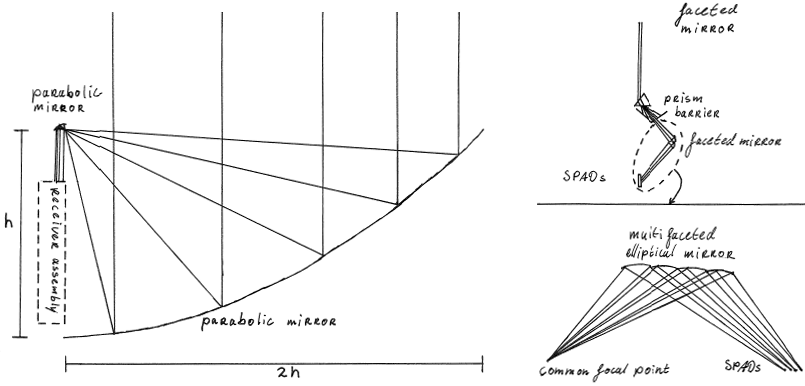
\includegraphics[scale = 0.5]{chapters/img/DiagramReceiverGeneral.png}
\caption{Receiver optics overview}
\label{fig:receiver_overview}
\end{figure} 

\subsection{\ac{SPAD}}
	\label{SPAD}
introduction

\subsubsection{Avalanche Diodes}
\label{diodes}	
Essentially, a \ac{SPAD} is a reversed biased \textit{p-n junction} that operates at a voltage level above the breakdown voltage. At this bias, the electric field is so high that a single charge carrier injected into the depletion layer can trigger a self-sustaining avalanche. The current rises swiftly (nanoseconds or subnanosecond rise time) to a macroscopic steady level in the milliampere range. Bias supply voltage Va exceeds breakdown voltage (non-destructive and reversible process) Vb by an amount called the \textit{excess bias voltage} $V_e = (V_a - V_b)$, which has a determining influence on detector performance. Actually, the value of the ratio $\frac{V_e}{V_b}$ is important, not the value of $V_e$ alone, because the performance is related to the excess electric field above breakdown level.  

If the primary carrier is photogenerated, the leading edge of the avalanche pulse marks the arrival time of the detected photon. The current continues to flow until the avalanche can be quenched by lowering the bias voltage to the breakdown voltage ($V_b$) or below. For a photon to be detected, not only must it be absorbed in the detector active volume and generate a primary carrier (more precisely, an electron-hole pair, i.e. \textit{an exciton}), it is also necessary that the primary carrier succeeds in triggering an avalanche. The efficiency of photon detection thus increases with excess bias voltage $V_e$, since higher electric field gradient enhances the triggering probability.   

As it happens in \ac{PMT}s, thermal generation effects produce current pulses even in the absence of illumination, and the Poissonian fluctuation of the dark counts represents the internal noise source of the detector. \textit{Dark-count rate} includes primary and secondary pulses. \textit{Primary dark pulses} are due to carriers thermally generated in the \acs{SPAD} junction, so that the count rate increases with the temperature as does the dark current in ordinary photodiodes. The rate also increases with $V_e$ because of field-assisted enhancement of the emission rate from generation centers and an increase in triggering probability. \textit{Secondary dark pulses} are due to afterpulsing effects that may strongly enhance the total dark-count rate. During avalanche some carriers are captured by deep levels in the junction depletion layer and subsequently released with a statistically fluctuating delay. Released carriers can retrigger the avalanche, generating afterpulses correlated with a previous avalanche pulse. The number of carriers captured during the avalanche pulse increases with the total number of carriers crossing the junction, that is, with the total charge of the avalanche pulse. Therefore afterpulsing increases with the delay of avalanche quenching and the current intensity, which is proportional to excess bias voltage $V_e$.

\begin{figure} [ht]
\centering
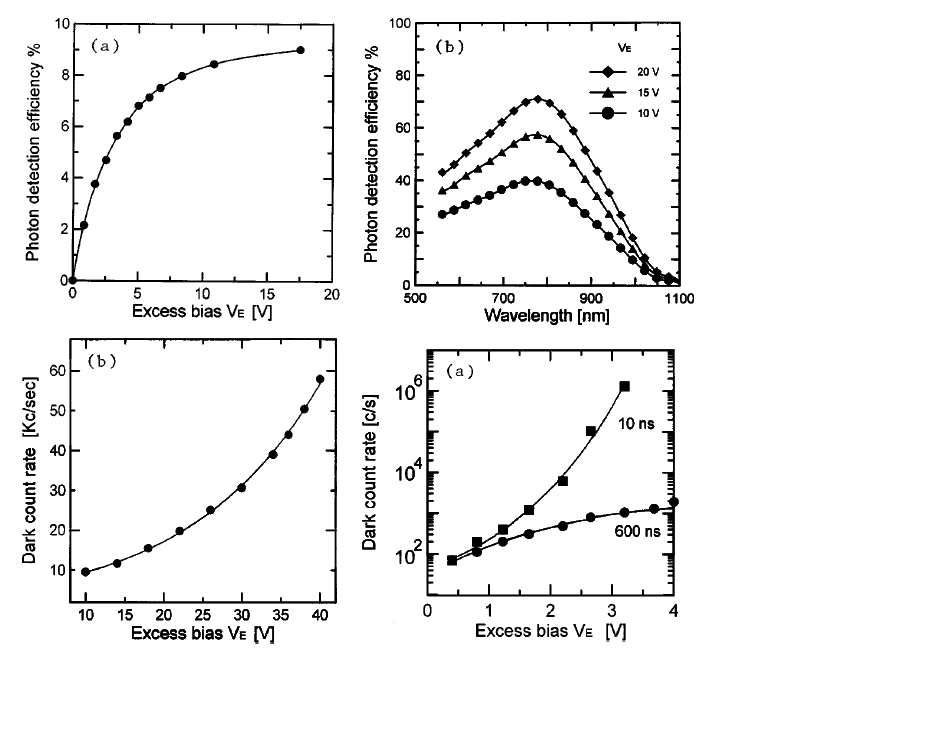
\includegraphics[scale=0.8]{chapters/img/SPAD_Ve_functions.png}	
\caption{\acs{SPAD} parameters diagrams }
\label{spad}
\end{figure}

\subsubsection{Quenching Circuits}
\label{AQC}
The bias voltage is then restored, in order to be able to detect another photon. 	
 

\subsection{Prism design}
\label{prism}
Before the prism is taking into consideration, the optical filter is also considered as an option, which is more simple than prism and barriers. The optical filters bandwidth accuracy are in terms of several docades of nano meters(minimum 10nm\cite{optical_filter}), which is not acceptable since the objective is to filter out all noisy light except wavelength around 473nm. Meanwhile, the transmission is another problem for normal optical filters, which have much lower value(around 50\%) for smaller bandwidth(10nm to 20nm) and higher value(around 90\%) for larger bandwidth(more than 30nm), but prism can has higher transmission as 97\% for specified glass material.

The figure \ref{fig:prism} on page \ref{fig:prism} gives an overview of the receiver optics after the second parabolic mirror. the prism is used to filter out all the noisy light except wavelength 472[nm] to 474[nm]. The prism system needs to be accurate enough to perform the filtering in limited distance. The design contains the type of prism glass material, the incident angle($\alpha$), prism apex angle($A$) and distance between prism and barriers. They will be treated one by one.

\begin{figure}[ht!]
\centering
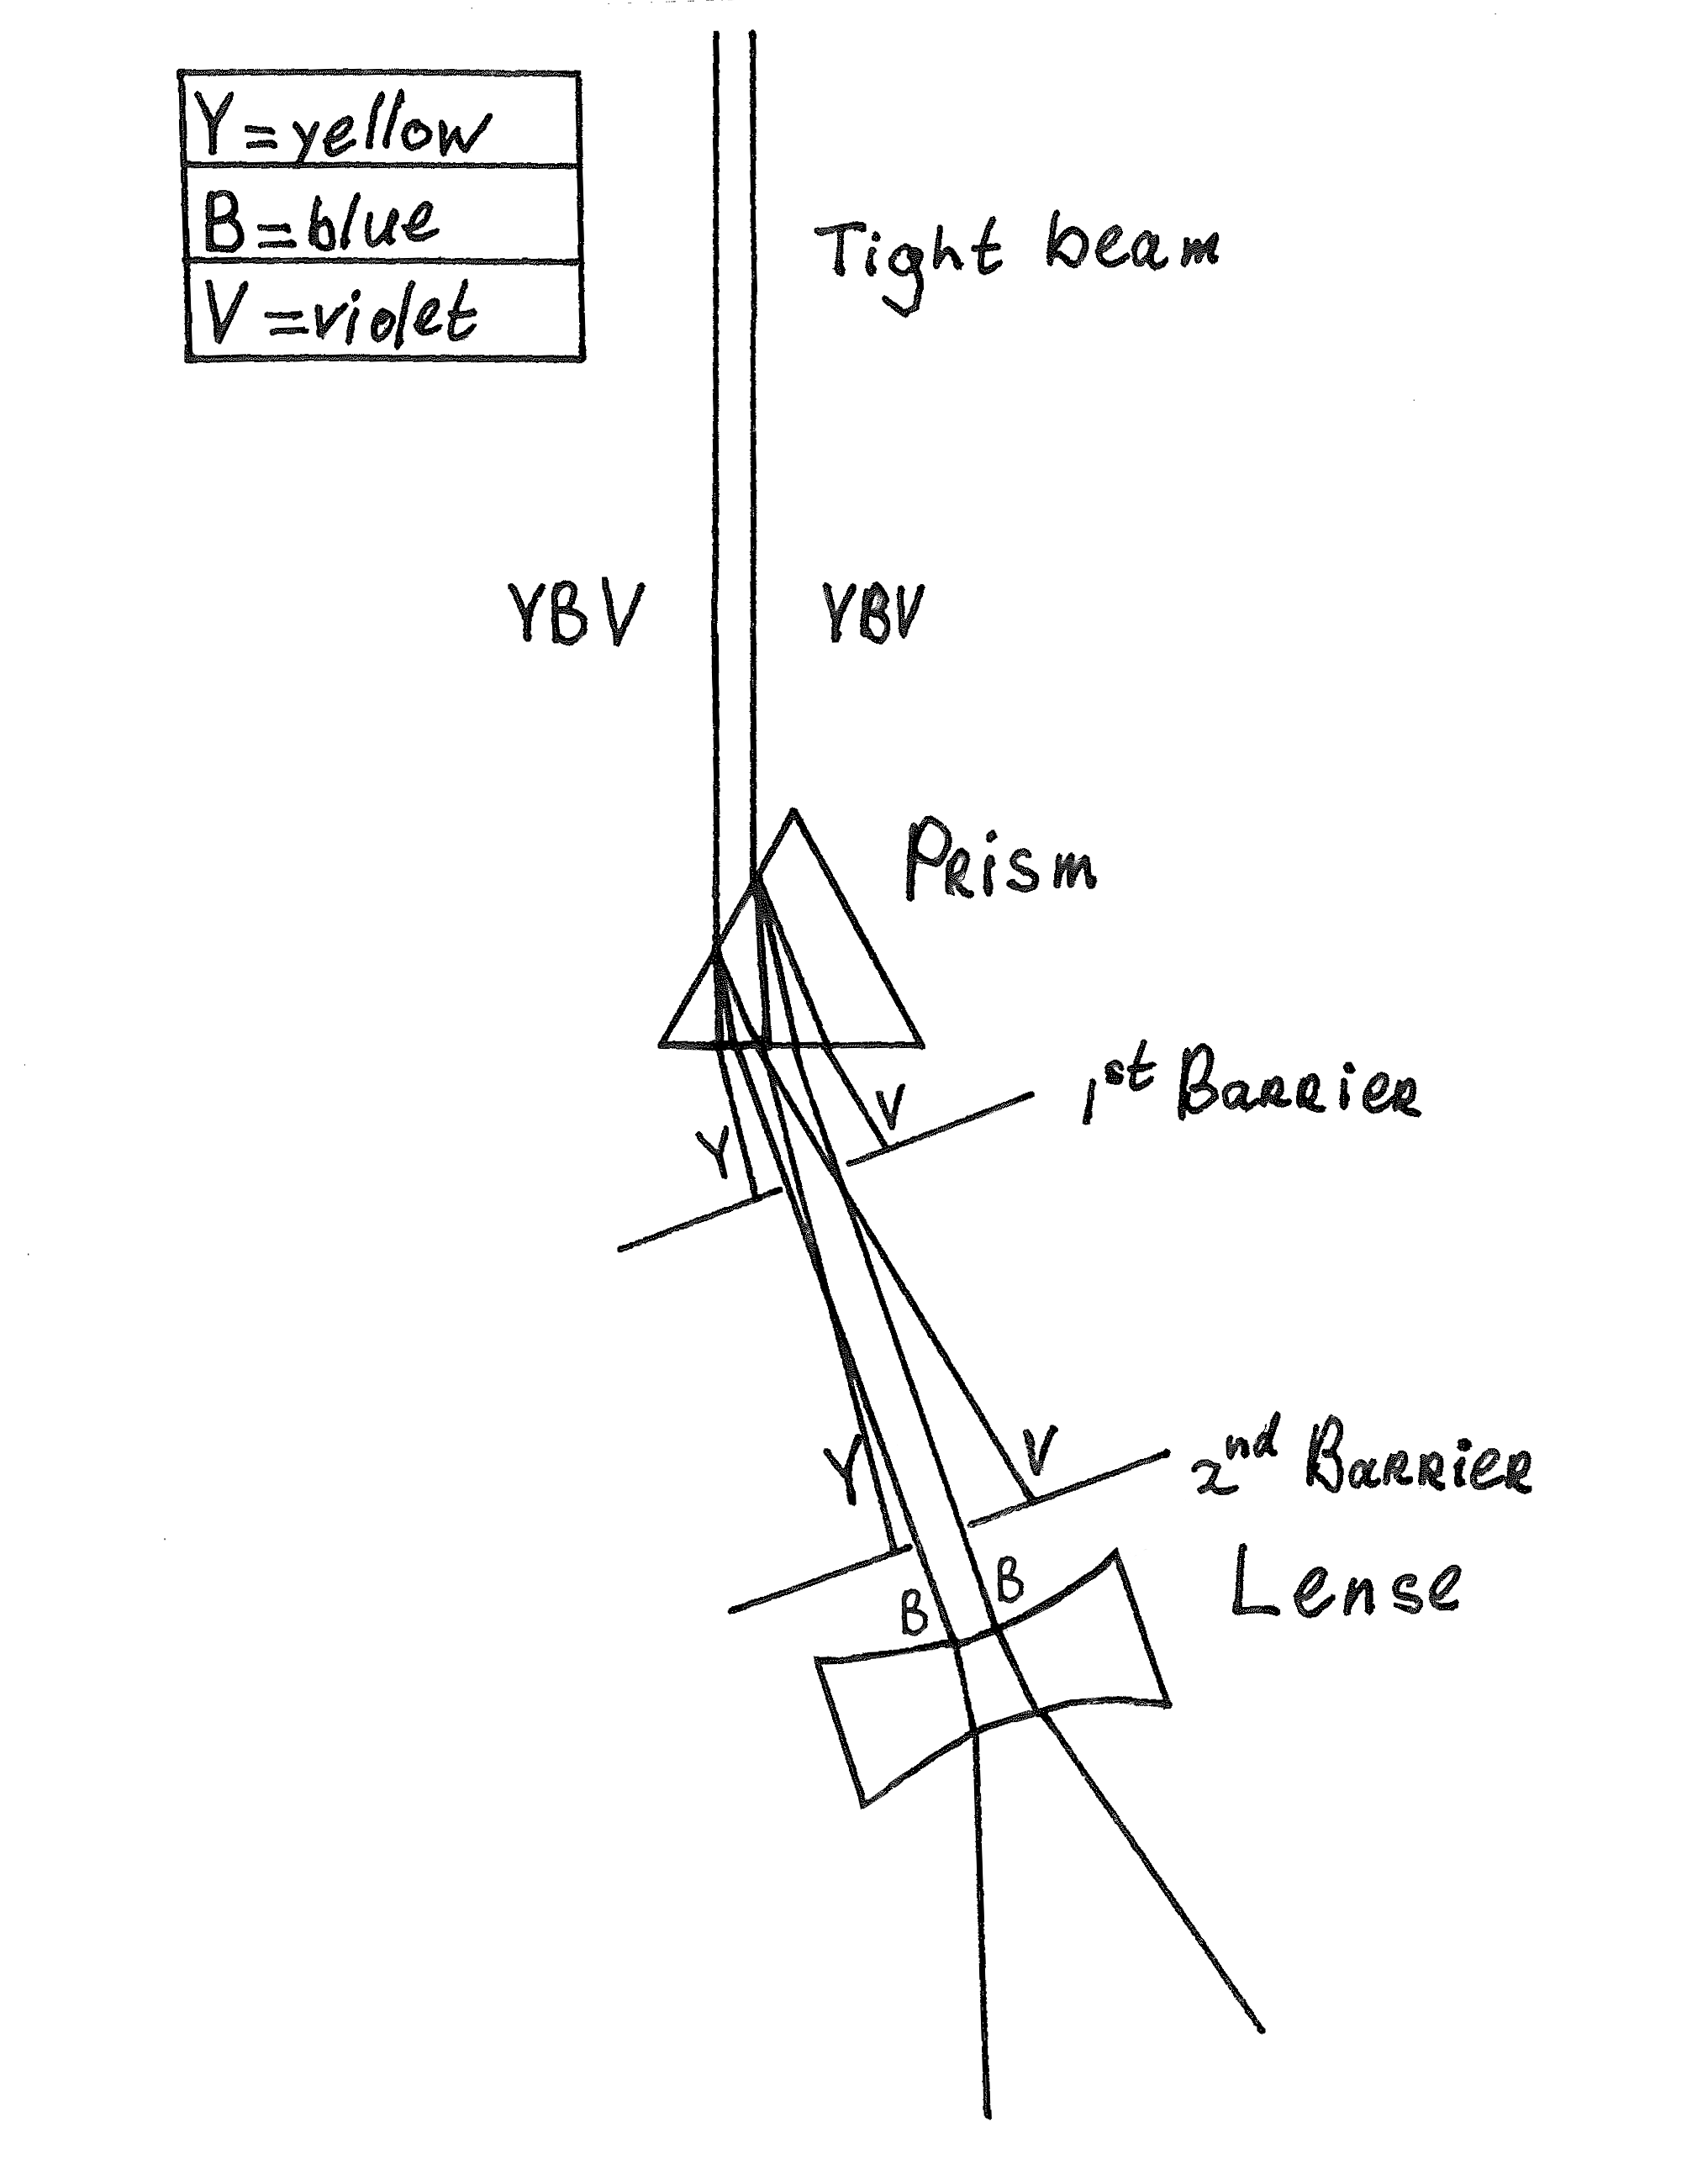
\includegraphics[scale = 0.8]{chapters/img/Prism.png}
\caption{Receiver prism filter overview}
\label{fig:prism}
\end{figure} 


\begin{figure}[ht!]
\centering
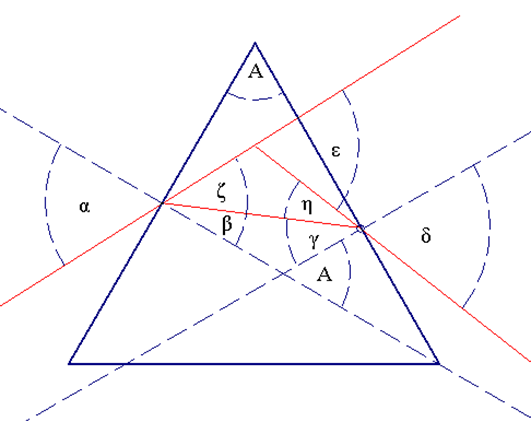
\includegraphics[scale = 0.8]{chapters/img/Prism2D.png}
\caption{Prism angles define in 2D}
\label{fig:prism2D}
\end{figure} 
In figure \ref{fig:prism2D} on page \ref{fig:prism2D}, the deviation angle $\epsilon$ can be calculated using the formula\cite{prism_angle_calculation}:
\begin{equation}
\label{epsilon}
\epsilon = \alpha - A + sin^{-1}(sin(A)\sqrt{n^2 - (sin(\alpha))^2} - cos(A)sin(\alpha))
\end {equation}
The key requirement to design the prism is to maximize the $\frac{d\epsilon}{d\lambda}$,  because for wavelength 473[nm] larger $\frac{d\epsilon}{d\lambda}$ leads to smaller distance between prism and barriers as well as the risk. The equation \ref{epsilon} indicates that the deviation angle($\epsilon$) is a function of A, $\alpha$ and n. From Sellmeier formula\cite{prism_book}, the index of refraction n can be calculated as:
\begin{equation}
\label{index_refraction}
n^2 - 1 = \frac{a_{1}\lambda^2}{\lambda^2-b_{1}} + \frac{a_{2}\lambda^2}{\lambda^2-b_{2}} + \frac{a_{3}\lambda^2}{\lambda^2-b_{3}}
\end {equation}
In the equation \ref{index_refraction}, $a_{1}, a_{2}, a_{3}$ and $b_{1}, b_{2}, b_{3}$ are the dispersion coefficients, which have different values for different glasses. In this case, the most 17 common prism glasses from Schott\cite{prism_material}\cite{prism_book} company are analyzed. Since it is difficult to calculate $\frac{d\epsilon}{d\lambda}$ analytically, $\Delta\epsilon$ due to wavelength 472[nm], 473[nm] and 474[nm] can be obtained by inserting arbitrary A and $\alpha$, which is actually the $\frac{d\epsilon}{d\lambda}$ because the wavelength difference is only 1[nm] of each. During the calculation, no matter what values are given to A and $\alpha$, SF11 glass always has the maximum value of $\Delta\epsilon$ which means it is the optimal glass material. Meanwhile, SF11 glass also has an internal transmittance of 97\% for wavelength around 473[nm], which is acceptable. Next step is to determine the prism apex angle(A) and the incident angle($\alpha$). The prism apex angle is defined as 60 degrees because which gives the most average value for $\Delta\epsilon$. Meanwhile, this kind of euqilateral prisms are also referred to as dispersing prisms used for wavelength separating applications(see figure \ref{fig:prism_equilateral} on page \ref{fig:prism_equilateral}). 

\begin{figure}[ht!]
\centering
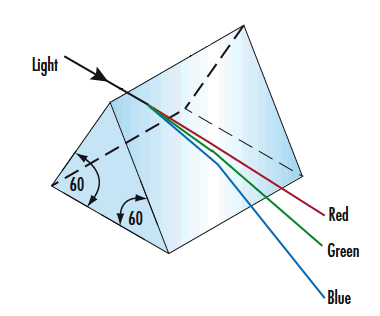
\includegraphics[scale = 0.8]{chapters/img/prism_equilateral.png}
\caption{Equilateral prism for wavelength separating applications}
\label{fig:prism_equilateral}
\end{figure}

To select the correct incident angle, the figure \ref{fig:prism_alpha} on page \ref{fig:prism_alpha} is used. In the figure, the blue line has the asymptote about $\alpha = 54[deg]$. To avoid the asymptote, $\alpha = 55[deg]$ is selected as the incident angle, which leads to $\epsilon = 76[deg]$ and $\Delta\epsilon = 2.1432[mrad]$. The figure \ref{fig:SF11} is the calculation in the excel sheet. There are two $\Delta\epsilon$ in the calculation, and $\Delta\epsilon1 = \epsilon(472[nm]) - \epsilon(473[nm])$ meanwhile $\Delta\epsilon2 = \epsilon(473[nm]) - \epsilon(474[nm])$. The driving $\Delta\epsilon$ is the smaller one, since it is the minimum requirement. Taking $\Delta\epsilon = 2.1432[mrad]$ into further calculation, in order to separate wavelength 472[nm], 473[nm] and 474[nm], barrier radius(or beam width) 1[mm] leads to distance 466.7[mm] between prism and barrier. To short the distance, more concentrated beam is needed from parabolic mirror. The figure \ref{fig:prism_final} on page \ref{fig:prism_final} shows the final values of all angles.

\begin{figure}[ht!]
\centering
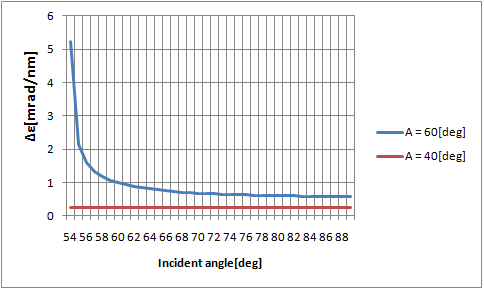
\includegraphics[scale = 1.2]{chapters/img/prism_alpha.png}
\caption{Plot of $\Delta\epsilon$ due to different incident angles}
\label{fig:prism_alpha}
\end{figure}

\begin{figure}[ht!]
\centering
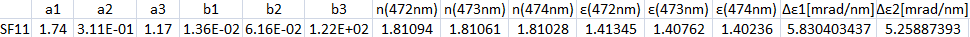
\includegraphics[scale = 0.8]{chapters/img/SF11.png}
\caption{Glass 'SF11' calculations}
\label{fig:SF11}
\end{figure}

\begin{figure}[ht!]
\centering
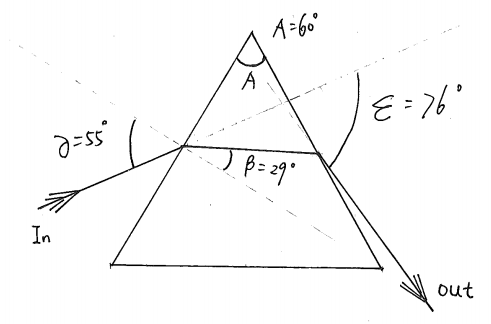
\includegraphics[scale = 0.8]{chapters/img/prism_final.png}
\caption{Overview of all angles}
\label{fig:prism_final}
\end{figure}

\subsection{Summary}
\label{sum}
The table \ref{tab:receiverbudget} on page \ref{tab:receiverbudget} is the budget breakdown including mass, cost and power consumption. It is obvious that the \acs{SPAD} is the main expense which is estimated by one of the developers. $4666530 FY00\$$ at the end is the final cost convert to fiscal year 2000. To be Clear, the large parabolic mirror is used to collect the reflected photons and the small parabolic mirror is used to create parallel tight beam before the prism. Flat mirrors are used after the prism to focus the light on faceted mirror.

\begin{table}[ht!]
\begin{tabular}{l | c | c c | c c | c }
Components         & Number & Mass & Cost      & Total mass & Total cost & Power\\ 
                   &        & [g]  & [Dollar]  & [g]        &[Dollar]    & [W]  \\ \hline\hline
Parabolic mirror(large)   & 1      & 100  & 7000      & 100        & 7000       &  0   \\
Parabolic mirror(small)   & 1      & 10   & 1500      & 10         & 1500       &  0   \\
Faceted mirror     & 1      & 30   & 3000      & 30         & 3000       &  0   \\ 
Flat mirror        & 5      & 10   & 500       & 50         & 2500       &  0   \\
\acs{SPAD}         & 1      & 10   & 5700000   & 10         & 5700000    &  0   \\
Prism              & 1      & 10   & 1500      & 10         & 1500       &  0.1 \\ 
Diverge lens       & 1      & 10   & 1000      & 10         & 1000       &  0   \\ \hline
Total              &        &      &           & 220        & 5716500    &  0.1 \\
                   &        &      &           &            & 4666530 FY00\$ &
\end{tabular}
\caption{Buget breakdown for receiver payload}
\label{tab:receiverbudget}
\end{table}